\chapter{Технологическая часть}

\section{Выбор средств реализации}
Для программной реализации алгоритма использовалась среда разработки Visual Studio 2022, язык программирования, на котором была выполнена реализации алгоритмов --- C++.
Для компиляции кода использовался компилятор MSVC. Исследование проводилось на ноутбуке (64--разрядная операционная система, процессор x64, частота процессора 3.1~ГГц, модель процессора 12th Gen Intel(R) Core(TM) i5-12500H, оперативная память 16~ГБ)
\section{Реализация алгоритмов}
В листинге \ref{list1} представлена программная реализация описанных алгоритмов.

\begin{lstlisting}[label = list1, caption = Программная реализация описанных алгоритмов]
#include <fstream>
#include <string>
#include <string_view>
#include <iostream>
#include <map>
#include <vector>
#include <algorithm>
#include <queue>
#include <filesystem>
#include <bitset>


int ROWS = 0;
int COLUMNS = 0;
int GEN_COL = 0;
int USEFUL = 0;
int X = 0;

using my_value_t = std::pair<std::string, size_t>;
using my_container_t = std::vector<my_value_t>;

struct Node {
	std::string name;
	Node* parent;
	Node* left_child;
	Node* right_child;
	
	Node(std::string nm, Node* prt, Node* lchild = nullptr, Node* rchild = nullptr) :
	name(nm), parent(prt), left_child(lchild), right_child(rchild) {}
	
	Node(std::string nm) : name(nm), parent(nullptr), left_child(nullptr), right_child(nullptr) {}
};

class HuffmanTree {
	Node* root = nullptr;
	std::vector<char> letters;
	
	public:
	void get_codes(std::string name, Node* current_node, std::map<char, std::string>& table) {
		if ((current_node->left_child == nullptr) and (current_node->right_child == nullptr)) {
			table[current_node->name[0]] = name;
			return;
		}
		if (current_node->left_child) {
			get_codes(name + "0", current_node->left_child, table);
		}
		if (current_node->right_child) {
			get_codes(name + "1", current_node->right_child, table);
		}
	}
	
	void set_letters(const std::vector<char>& buf) 
	{
		letters.clear();
		letters.reserve(buf.size());
		letters.append_range(buf);
	}
	
	template <typename CMP>
	void make_tree(std::priority_queue<my_value_t, my_container_t, CMP>& q)
	{
		my_value_t left, right;
		size_t total_weight;
		Node* tmp_root = nullptr;
		Node* left_child;
		Node* right_child;
		std::map<std::string, Node*> storage;
		
		while (q.size() > 1)
		{			
			right = q.top();
			q.pop();
			
			left = q.top();
			q.pop();
			
			tmp_root = new Node(left.first + right.first);
			
			total_weight = right.second + left.second;
			right_child = storage.contains(right.first) ? storage[right.first] : new Node(right.first, tmp_root);
			left_child = storage.contains(left.first) ? storage[left.first] : new Node(left.first, tmp_root);
			
			q.push(std::make_pair(left.first + right.first, total_weight));
			
			tmp_root->left_child = left_child;
			tmp_root->right_child = right_child;
			
			storage.insert(std::make_pair(left.first + right.first, tmp_root));
		}
		root = tmp_root;
	}
	
	auto create_table(std::vector<my_value_t> q)
	{
		std::ofstream file_table;
		std::map<char, std::string> table;
		
		file_table.open("table.txt", std::ios::out);
		
		get_codes("", root, table);
		
		std::cout << "\n";
		for (auto el : q) {
			//std::cout <<  el.first << " " << table[el.first[0]] << " " << el.second * (table[el.first[0]].size()) << "\n";
			X += el.second * (table[el.first[0]].size());
		}
		USEFUL = X % 8;
		//std::cout << "\n1 ----- X - " << X  << "USE - " << USEFUL;
		
		file_table << ROWS << std::endl;
		file_table << COLUMNS << std::endl;
		for (const auto& item : table) {
			std::cout << item.first << ":" << item.second << std::endl;
			file_table << item.first << ":" << item.second << std::endl;
		}
		file_table << X;
		file_table.close();
		return table;
	}
	
	void code(std::string flow, std::map<char, std::string>& table) {
		std::ofstream file_b;
		
		file_b.open("coded.bin", std::ios::binary);

		std::vector<uint8_t> packed_data;
		uint8_t byte = 0;
		int bit_count = 0;
		
		std::string coded_flow;

		int A = 0;
		A = USEFUL;
		while (coded_flow.length() < 8) {
			if (USEFUL == 0) {
				coded_flow += "0";
				continue;
			}
			coded_flow += std::to_string((USEFUL % 2));
			USEFUL /= 2;
		}
		std::reverse(coded_flow.begin(), coded_flow.end());
		//USEFUL = A;
		
		int i = 0;
		for (int ch : flow) {
			i++;
			coded_flow += table[ch];
		}

		byte = 0;
		
		for (char bit : coded_flow) {
			byte = (byte << 1) | (bit - '0');
			bit_count++;
			if (bit_count == 8) {
				packed_data.push_back(byte);
				byte = 0;
				bit_count = 0;
			}
		}
		
		if (bit_count > 0) {
			byte <<= (8 - bit_count);
			packed_data.push_back(byte);
		}
		
		std::ofstream file("coded.bin", std::ios::binary);
		if (file.is_open()) {
			file.write(reinterpret_cast<const char*>(packed_data.data()), packed_data.size());
			file.close();
		}
		
		file_b.close();
	}
	
};

int main() {
	setlocale(LC_ALL, "rus");
	
	std::vector<my_value_t> copy;
	
	std::string filename = "test_2.txt";
	
	std::string data;
	std::ifstream file;
	std::string gen_string;
	
	std::vector<char> all_letters;
	
	std::map<char, size_t> letters;
	std::vector<std::pair<char, size_t>> letters_vec;
	auto comp = [](const my_value_t& nd_1, const my_value_t& nd_2) {return nd_1.second > nd_2.second; };
	
	std::priority_queue<my_value_t, my_container_t, decltype(comp)> letters_q{ comp };
	
	file.open(filename, std::ios::in);
	
	while (getline(file, data)) {
		if (ROWS == 0) {
			if (isdigit(data[0])) {
				ROWS = std::atoi(data.c_str());
			}
		}
		else if (COLUMNS == 0) {
			if (isdigit(data[0])) {
				COLUMNS = std::atoi(data.c_str());
			}
		}
		else {
			for (int i = 0; i < data.size(); ++i) {
				if (letters.contains(data[i]))
				letters[data[i]]++;
				else
				letters[data[i]] = 1;
				GEN_COL++;
			}
			gen_string += data;
		}
	}
	
	
	for (const auto& item : letters){
		letters_q.push(std::make_pair(std::string(1, item.first), item.second));
		copy.push_back(std::make_pair(std::string(1, item.first), item.second));
		all_letters.push_back(item.first);
	}
	
	HuffmanTree tree;
	tree.make_tree(letters_q);
	tree.set_letters(all_letters);
	
	data.clear();
	
	file.close();
	
	auto table = tree.create_table(copy);
	
	tree.code(gen_string, table);
	
	std::ifstream file_out_b("coded.bin", std::ios::binary);
	
	std::istreambuf_iterator<char> start{ file_out_b }, end;
	
	std::vector<uint8_t> packed_data(start, end);
	file_out_b.close();
	
	std::string binary_data_1;
	std::string binary_data_2;
	int cn = 0;
	int byte_in_f = X / 8;
	std::string local_st;
	
	int USE = 0;
	for (uint8_t byte : packed_data) {
		if (cn == 0) {
			binary_data_1 += (std::bitset<8>(byte).to_string());
			std::reverse(binary_data_1.begin(), binary_data_1.end());
			for (int i = 0; i < binary_data_1.length(); i++) {
				if (binary_data_1[i] == '1') USE += pow(2, i);
			}
			std::reverse(binary_data_1.begin(), binary_data_1.end());
		}
		else {
			if ((byte_in_f + 1) == cn) {
				local_st = (std::bitset<8>(byte).to_string());
				for (int i = 0; i < USE; i++) {
					binary_data_2 += local_st[i];
				}
				break;
			}
			binary_data_2 += (std::bitset<8>(byte).to_string());
		}
		cn++;
	}
	
	std::string buff;
	
	for (int i = 0; i < binary_data_2.length(); i++) {
		if ((i % 8) == 0) std::cout << " ";
		std::cout << binary_data_2[i];
	}
	
	std::cout << "\n";
	
	for (auto el : binary_data_2) {
		buff += el;
		for (auto [key, val] : table) {
			if (val == buff) {
				std::cout << key;
				buff.clear();
			}
		}
	}
}
\end{lstlisting}

\section{Тестирование программы}
В таблицах \ref{tab:tests}, \ref{tab:tests2} представлены описания тестов по методологии чёрного ящика, все тесты пройдены успешно.

\begin{table}[htbp]
	\centering
	\caption{Описание тестов по методологии чёрного ящика}
	\begin{tabular}{|p{0.05\linewidth}|p{0.22\linewidth}|p{0.2\linewidth}|p{0.2\linewidth}|p{0.2\linewidth}|}
		\hline
		№ & \textbf{Описание теста} & \textbf{Входные данные} & \textbf{Ожидаемый результат} & \textbf{Полученный результат} \\
		\hline
		
		\textbf{1} 
		& проверка кодирования матрицы с элементами меньше десяти
		&Файл 1:3 \newline 2 \newline 1 0/\newline 2 3/\newline 4 0/
		& :10 \newline/:01 \newline0:000 \newline1:0011 \newline2:110 \newline3:0010 \newline4:111
		&  :10 \newline/:01 \newline0:000 \newline1:0011 \newline2:110 \newline3:0010 \newline4:111\\
		\hline
		
		\textbf{2} 
		& проверка кодирования матрицы с элементами больше десяти
		&Файл 1: \newline3 \newline3 \newline 10 0 12/\newline 12 23 34/\newline 41 30 1/
		& :01 \newline/:0000  \newline0:100  \newline1:11  \newline2:001  \newline3:101 \newline4:0001
		& :01 \newline/:0000  \newline0:100  \newline1:11  \newline2:001  \newline3:101 \newline4:0001\\
		\hline
		
		\textbf{3} 
		& проверка кодирования матрицы с элементами меньше нуля
		&Файл 1: \newline3 \newline3 \newline -10 0 -12/\newline 12 -23 34/\newline -41 30 -1/
		& :10 \newline-:010 \newline/:110 \newline0:011 \newline1:001 \newline2:0000 \newline3:111 \newline4:0001
		& :10 \newline-:010 \newline/:110 \newline0:011 \newline1:001 \newline2:0000 \newline3:111 \newline4:0001\\
		\hline
	\end{tabular}
	\label{tab:tests}
\end{table}

\begin{table}[htbp]
	\centering
	\caption{Описание тестов по методологии чёрного ящика}
	\begin{tabular}{|p{0.05\linewidth}|p{0.22\linewidth}|p{0.2\linewidth}|p{0.4\linewidth}|}
		\hline
		№ & \textbf{Описание теста} & \textbf{Входные данные} & \textbf{Содержимое файла}\\
		\hline
		
		\textbf{1} 
		& проверка кодирования матрицы с элементами меньше десяти
		&Файл 1:3 \newline 2 \newline 1 0/\newline 2 3/\newline 4 0/
		& 1101000111000001110100010011111\-000001\\
		\hline
		
		\textbf{2} 
		& проверка кодирования матрицы с элементами больше десяти
		&Файл 1: \newline3 \newline3 \newline 10 0 12/\newline 12 23 34/\newline 41 30 1/
		& 00000101 11100011 00011100 10000110 01010011 01011010 00100000 00111011 01100011 10000\\
		\hline
		
		\textbf{3} 
		& проверка кодирования матрицы с элементами меньше нуля
		&Файл 1: \newline3 \newline3 \newline -10 0 -12/\newline 12 -23 34/\newline -41 30 -1/
		& 00000001 01000101 11001110 01000100 00110001 00001001 00000111 10111000 11100100 00100110 11101110 01000111 0\\
		\hline
	\end{tabular}
	\label{tab:tests2}
\end{table}

\section{Примеры работы программы}
Снимки экрана \ref{1}, \ref{2}, \ref{3} c примером работы программы с входными данными соответствующими тестам описанным в таблице \ref{tab:tests}. 

{\centering
	
\includegraphics[scale = 0.6]{1}
	\captionof{figure}{Пример работы программы 1}
}
\label{1}
{\centering
	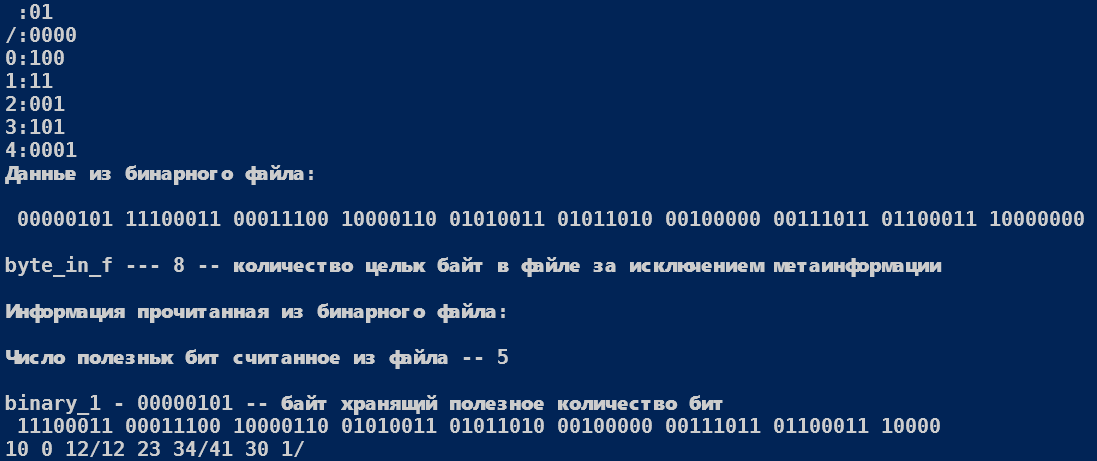
\includegraphics[scale = 0.6]{2}
	\captionof{figure}{Пример работы программы 2}
}
\label{2}
{\centering
	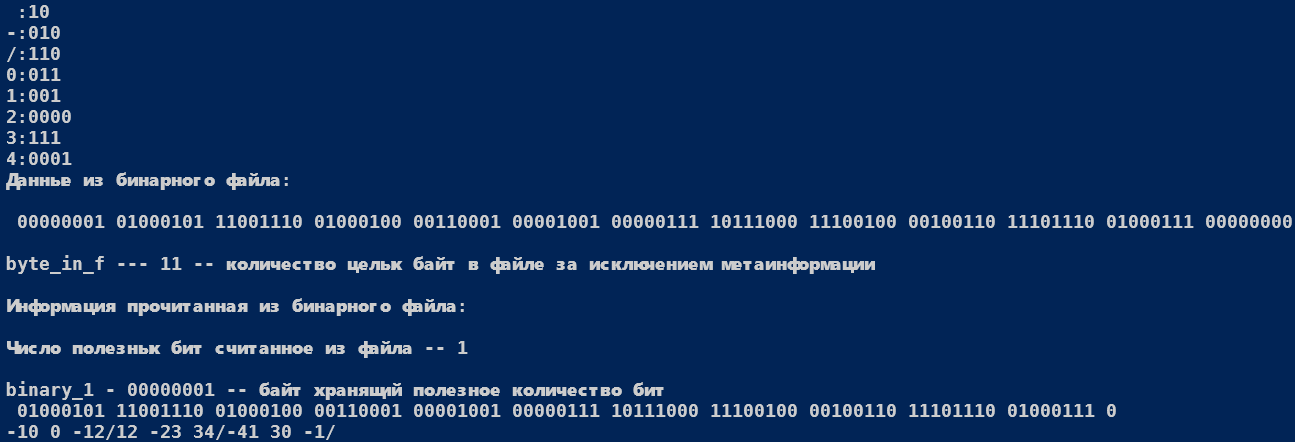
\includegraphics[scale = 0.505]{3}
	\captionof{figure}{Пример работы программы 3}
}
\label{3}
\clearpage
